\documentclass[12pt]{article}


\usepackage{geometry}
 \geometry{
 a4paper,
 left=20mm,
 right=20mm,
 top=10mm	
 }

\usepackage{amssymb}
\usepackage[utf8]{inputenc}
\usepackage{graphicx}
\usepackage{amstext}
\usepackage{amsmath}
\usepackage[section]{placeins}


\newtheorem{theorem}{Definice}


\title{BI-ZUM - Stavový prostor a jeho prohledávání, stromová expanze, náhodné prohledávání, prohledávání do hloubky a do šířky.}
\author{Vastl Martin}

\begin{document}
\maketitle
\author

Stavový prostor si lze představit jako graf, kde vrchol představuje nějaký popis stavu řešeného problému a hrany reprezentují akce a umožňují přechod mezi stavy. Příklady takových problému jsou např. hledání nejkratší cesty, symbolická integrace, a podobně. Množinu stavů značíme $S$ a množinu akcí $A$.

\begin{theorem}
Mějme stavový prostor $(S,A)$. Úloha prohledávání $(S,A)$ je zadána:
\begin{itemize}
\item počátečním stavem $I\in S$,
\item množinou koncových stavů $G\subseteq S$
\end{itemize}
\end{theorem}

\begin{theorem}
Nechť $(S,A)$ je stavový prostor a $s\in S$ je stav v tomto prostore. Řekneme, že stav $s'\in S$ je následníkem stavu s, pokud $(s,s')\in A$, tj. pokud existuje nějaká akce, která přesune stav $s$ do stavu $s'$.
\end{theorem}

Problém popsaný stavovým prostorem v praxi převádíme na jednu z následujících úloh:
\begin{itemize}
\item hledání cesty z počátečního do koncového stavu (nejkratší cesta, symbolická integrace i s postupem)
\item hledání cílového stavu (řešení sudoku, problém n dam)
\end{itemize}

\section{Stromová expanze}


\begin{theorem}
Uvažujme stavový prostor $X=(S,A)$ počáteční stav $I\in S$ a množinu koncových stavů $G \subseteq S$. Prohledávací strom $X$ je orientovaný kořenový strom s kořenem $I$, takový, každá cesta v tomto stromě se vyskytuje i v grafu $(S,A)$.
\end{theorem}

\begin{figure}[!htb]
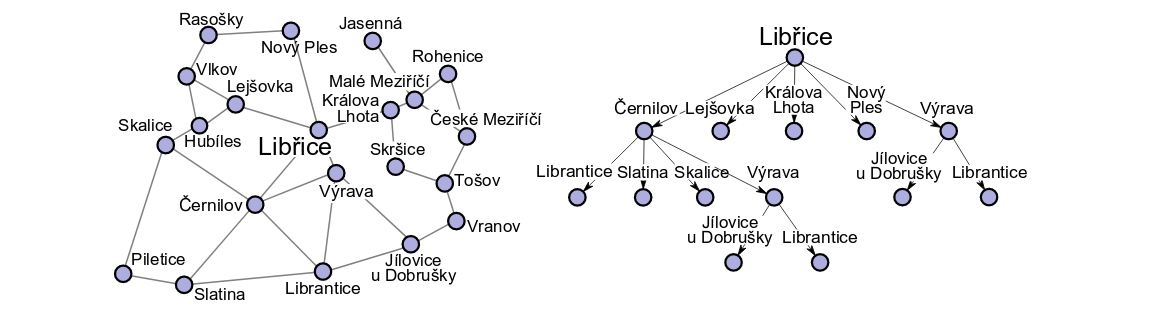
\includegraphics[width=\linewidth]{stromovaExpanze}
\end{figure}

\begin{figure}[!htb]
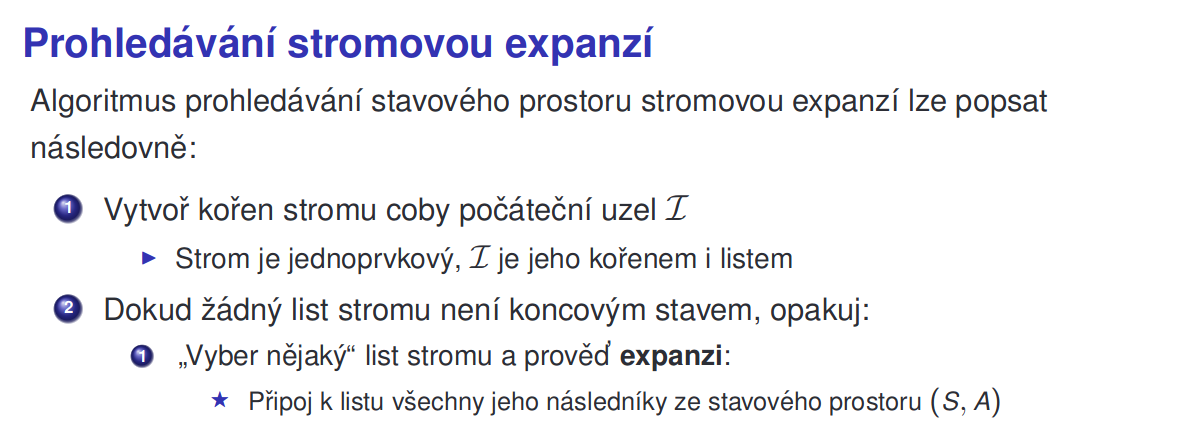
\includegraphics[width=\linewidth]{prohledavani}
\end{figure}

\begin{figure}[!htb]
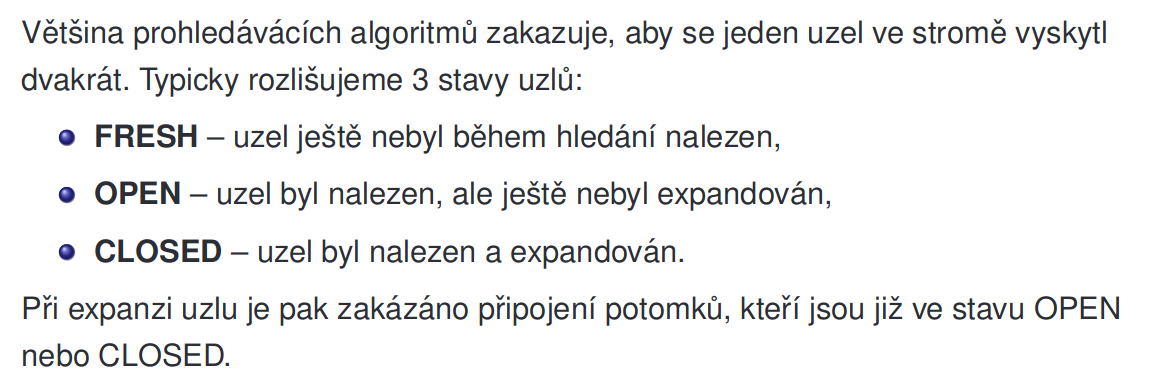
\includegraphics[width=\linewidth]{fresh-open-closed}
\end{figure}


\section{Náhodné prohledávání}
Náhodně prohledávání je takové prohledávání, které náhodně otevírá jednotlivé vrcholy stavového prostoru. Je možné, že nalezne neoptimální řešení.
\begin{figure}[!htb]
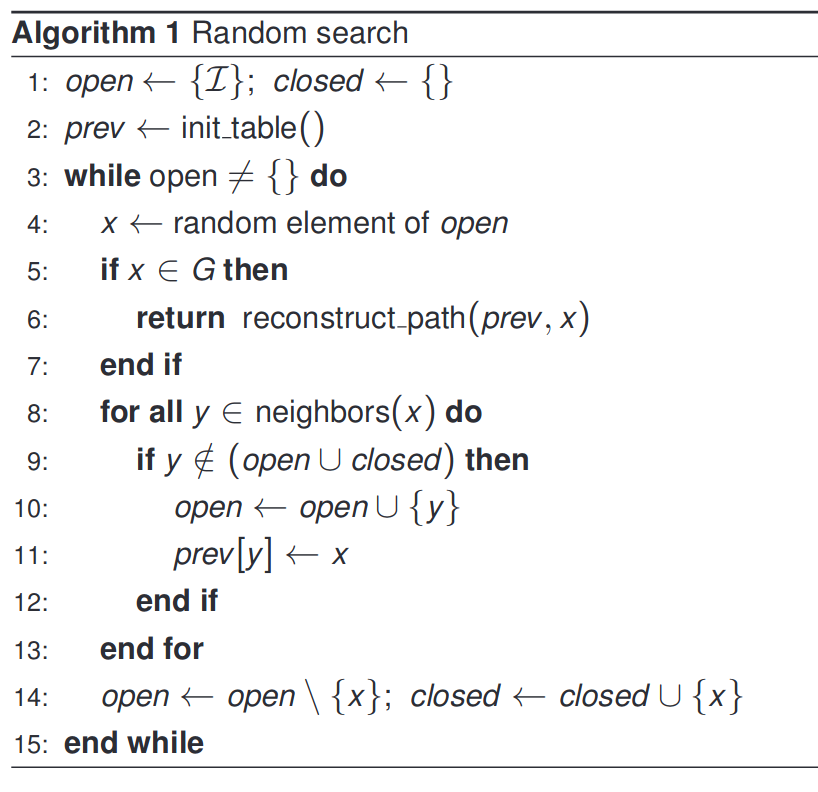
\includegraphics[width=0.5\linewidth]{random}
\end{figure}

\section{BFS}
BFS provádí expanzi postupně po jednotlivých patrech. Zaručuje, že výsledná cesta bude mít nejmenší možný počet hran. Jeho paměťová i výpočetní čas roste exponenciálně s délkou nejkratší cesty (co do počtu hran) cesty k cíli.
\begin{figure}[!htb]
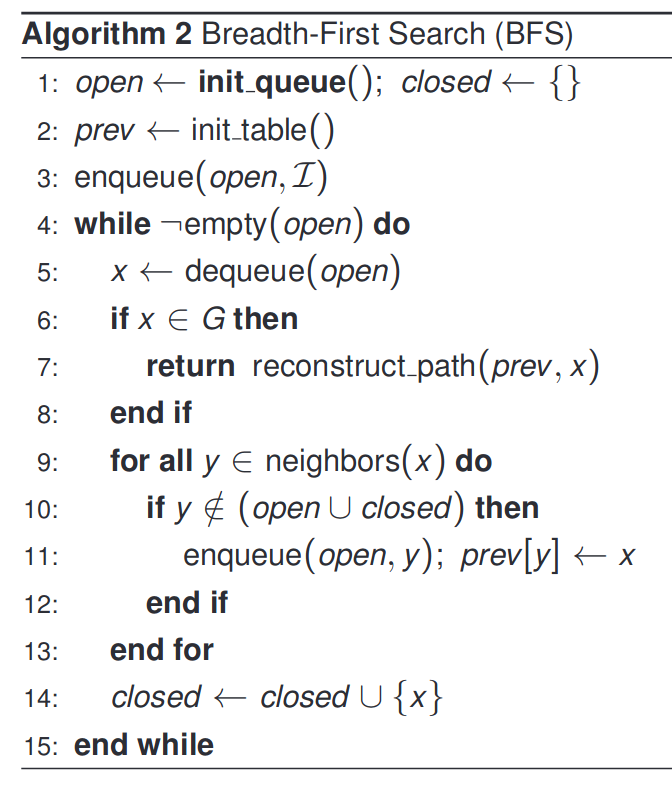
\includegraphics[width=0.5\linewidth]{bfs}
\end{figure}


\section{DFS}
DFS prochází stavový prostor a snaží se o co největší zanoření. Nemusí vždy najít nejkratší cestu, co se do počtu hran týká.
\begin{figure}[tb]
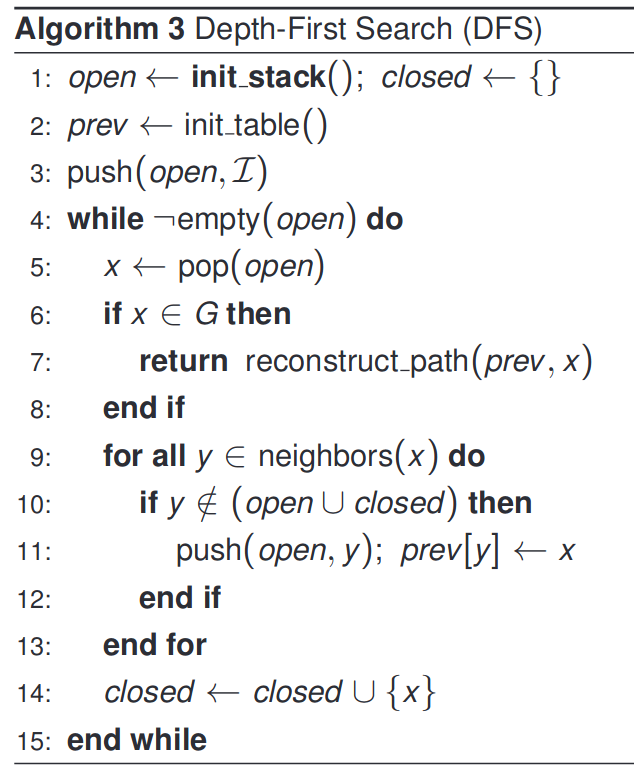
\includegraphics[width=0.5\linewidth]{dfs}
\end{figure}

\end{document}

















